\section{Model Development}
In this section we propose a CNN for encoding the direction of linear and angular movement observed between 2 frames, and a RNN to classify sequences of encoded movement as a gesture.
These models are to be used in tandem to classify semaphoric gestures performed, distinguishing between gesture made with the head and those made with a smartphone.
% script.processor.process_data('G:/Study/7', 1900)
% script.processor.process_data('G:/Study/6', 8900)
% script.processor.process_data('G:/Study/5', 9500)
% script.processor.process_data('G:/Study/4', 900)
% script.processor.process_data('G:/Study/3', 20000)
% script.processor.process_data('G:/Study/2', -320, attempt_0_override=-320)
% script.processor.process_data('G:/Study/1', 1000)
% script.processor.process_data('G:/Study/0', 3000)

% \subsection{The Proposed Models} % TODO: Drop /s if only one model % The Proposed System
% Both models then used to train HMM, evaluate which performs better
% In this section we shall propose two models for quantising the motion of the phone and position of the head, and a HMM to classify sequences of the encoded motion as specific gestures.
% Possibly one-hot encoding
% \nl\textbf{Modularity}\\
% Having a single model do many tasks
We opted to split the development of our model into two distinct models (the CNN and RNN) for 2 reasons.
The first was to reduce the observation space for the RNN, since the acceleration can be any value and the position of the face in the image also any range of values, within the boundaries of the image resolution.
To use them as raw inputs to an RNN would require a significant amount of data to ensure we have samples that cover the entire training space.
By first encoding the data we can reduce the possible training space.
The simplest way to perform this would be to quantise the data. This would involve reducing the resolution of the data, for example mapping all the angles of rotation into a smaller range, as was performed by \citeauthor{elmezain2008hidden} to convert the movement of a hand capture in a sequence of images to the angle of the movement~\cite{elmezain2008hidden}, reducing the possible input to their HMM to just 19 observable states.
We have decided to instead one-hot encode the motion of the head and phone. This reduces the possible states for two frames down to a 12x3 grid, where the columns are the degree of freedom.

The second reason  for the split was to reduce the memory requirements for the system.
An RNN requires a sequence of input in order or to predict an output. If we were to utilise a CNN atop the RNN, we would need to hold enough images in memory for the required input length of the RNN. The longer the input sequence is, the more images we would need. 2 Ways to get around this are to keep a short input sequence, reducing the amount of history that the RNN can learn and predict from; or we can reduce the image size, however reducing them too far can result in fewer features being extractable.
By splitting into two models, with distinct responsibilities, we only need to hold two images at a time in memory to encode the motion, and then hold onto the encodings for the second model's input sequence.

\subsection{Motion Encoding CNN Model}
% Want to reduce the possible observation states we need to learn for our classification HMM.
% \nl\textbfit{Classifier 1}\nl
% 2: Cascading motion encoder
%   No transfer learning
%   use YuNet to preprocess the image. 
%   - If no face found then return no encoding for face
%   - Else feed into NN to encode the motion
%   Acceleration encoded manually, just quantise and see if over given amount, then convert to encoding
\begin{figure*}
    \centering
    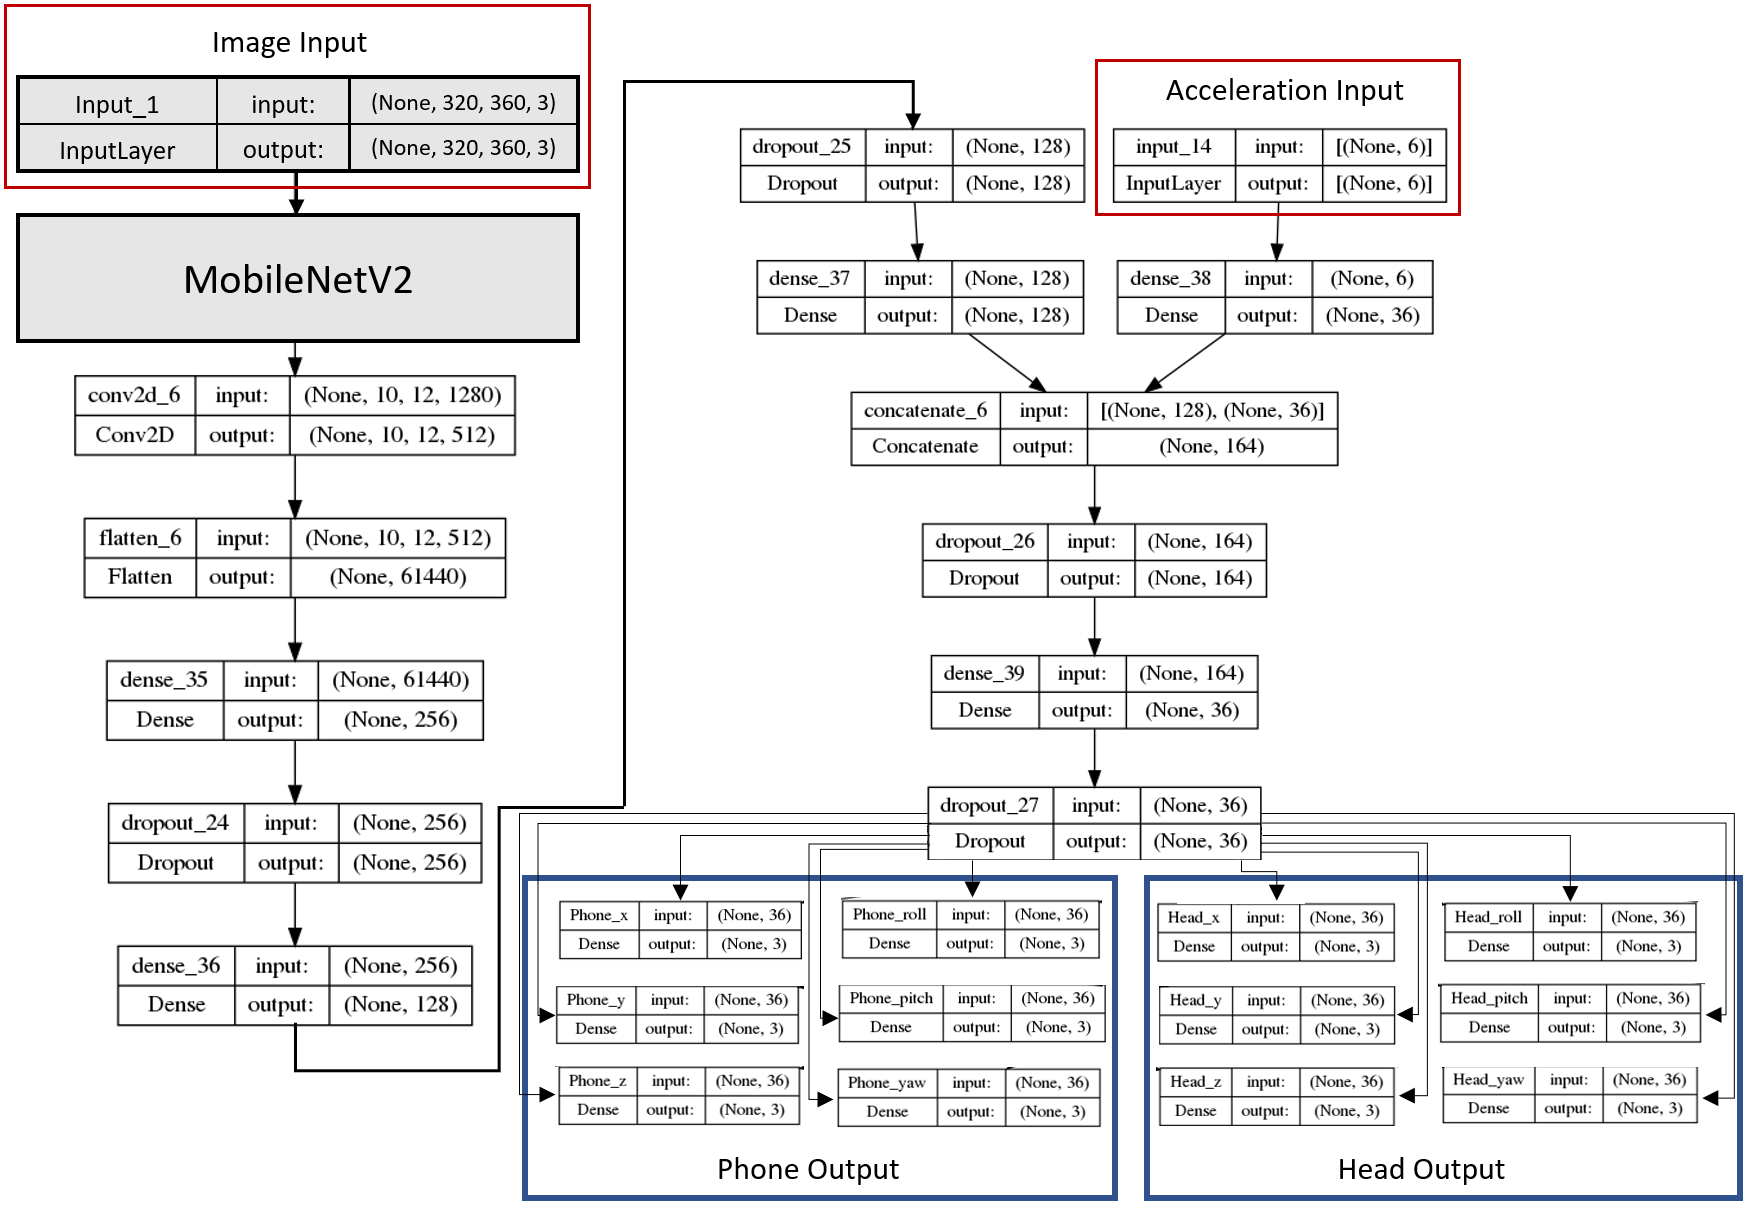
\includegraphics[width=0.95\textwidth]{figures/TL_Model_Clean.png}
    \caption{\label{fig:motion_encoder} Motion Encoder Model}
    \Description{Diagram of the motion encoder model, showing the image inputs feeding into the MobileNetV2 model, the acceleration input being joined with the output of the mobile net and subsequent dense layers, and the 12 expected output.}
\end{figure*}
First we propose a model for extracting the motion performed by the head and the phone.
Since this model requires extracting features from images, in order to learn and predict the motion of the head within the images, we elected to use a CNN.
To save on computation time and effort we employed transfer learning, a technique for extending upon an existing model with pre-initialised weights. For this we chose to use the MobileNetV2 network available within TensorFlow's Keras prebuilt models. We chose MobileNetV2 as, of the models available within Keras\footnote{A list of available models included within Keras for transfer learning can be found here: \url{https://keras.io/api/applications/}}, it strides a balance between size (14MB), accuracy (71.3\%), and CPU step inference time (25.9ms).
MobileNetV2 was trained on the ImageNet dataset\footnote{\url{https://www.image-net.org/}}, a dataset of millions of labelled images. These contain various classes, amongst them are people and faces.
By using just the CNN component of MobileNetV2 and freezing the weights, such that they are not updated during training, we should be able to utilise the features they have already learnt in order to process our image inputs, without needing to train a CNN from scratch.

\begin{figure}
    \centering
    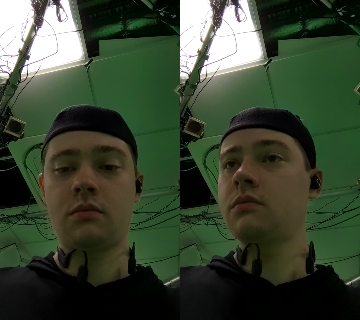
\includegraphics[width=0.4\textwidth]{figures/concat_input.png}
    \caption{\label{fig:concat_img} Concatenated Image Input For the Motion Encoder}
    \Description{Image composed of two input images that are used as input for the motion encoder.}
\end{figure}
Given we need the model to extract the motion of the head between two images, you may wonder why the input of the model accepts only a single RGB image with the dimensions $320x360x3$, as can be seen in the model graph \autoref{fig:motion_encoder}.
This is due to a limitation of TensorFlow/Keras, wherein using 2 of the same model for transfer learning fails due to layers from each model having the same name, resulting in the model graph being unable to compile. As such we were unable to have two branches utilising the MobileNetV2 to process the images individually. So to get around this issue we first stitch the images side-by-side, such that the older image is on the left, and the later image on the right, as shown in \autoref{fig:concat_img}.
This should not be an issue, as given the nature of CNNs, learned features are not dependent on location within the image, and as such features should still be extracted for both images. This also reduces the size of the model, given it does not need to have two copies of the same CNN.

Following the MobileNetV2 CNN, we add an additional couple of convolution layers, batch normalisation, and max pooling to reduce the parameters in the model, that need to be trained, before flattening the into a 1D tensor that will be concatenated with the acceleration input, starting the first layer of our Fully Connected Network (FCN).
The FCN layers are responsible for performing the classification based on the features extracted in the CNN. 
We opted to provide the acceleration as input into the model in order to allow the model to learn how the head pose changes with respect to acceleration.
We also have the model try to encode the motion of the phone, since we are providing the phone acceleration as input.
The output for this model is a total of 12 layers, each with 3 units which are encoded via a softmax activation function, which normalises the 3 values for each output, such that the most prediction that the model believes is most likely is the value closer to 1.

The model was implemented using TensorFlow's Keras Api.
The full model layers, excluding the MobileNetV2 CNN, can be seen in \autoref{fig:motion_encoder}.

% might encode one-hot instead, in which case take two sequential inputs and calculate the movement

% \nl\textbfit{Classifier 2}\nl
% % 2: NN using transfer learning (using image net model, which one?).
% %   Use tensorflow (work with current cuda and dependencies?) or pytorch?
% %   - 4 inputs, 2 images, 2 sets of acceleration data
% %     Images fed into own image net model, outputs into FCN and then both connected into FCN
% %     Acceleration fed into FCN, then joined with FCN of images
% %   Output one-hot encoded direction of motion for each DoF
% %   might be slow as re-processing previous image
% Our second proposed model we will be using transfer learning to extend an existing CNN trained on image net to predict the direction of motion, in each degree of freedom for both the head and phone, observed between two frames.
% We could try to emulate the YuNet model, and output the head pose and position, a lack of 
% One issue is lack of images not containing face, how to handle if no face detected?


\subsection{Gesture Classification RNN Model}
% Could have used an RNN bolted directly onto the back of the classifiers
\begin{figure}
    \centering
    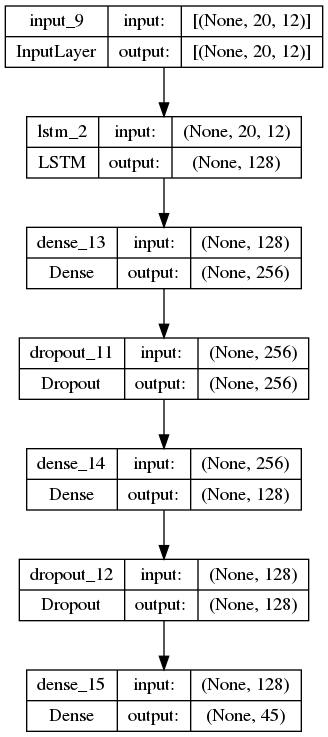
\includegraphics[width=0.25\textwidth]{figures/gesture_model.png}
    \caption{\label{fig:gesture_classifier} Gesture Classifier Model}
    \Description{Diagram of the gesture classifier model, showing the sequence input and one-hot encoded output layers.}
\end{figure}
Once we have our encoded motions, we can now look to classifying the sequence of these observations as gestures.
We elected to use an RNN for this task as, unlike a traditional Neural Network, it can hold onto state between elements of a sequence, allowing it to learn to recognise features within sequences. This is ideal as gesture is a sequence of motions, as long as the motions are correctly encoded and the sequence is long enough to envelop the motion duration, or at least the most significant motions within the gesture.

% \begin{figure}
%     \centering
%     \includegraphics[width=0.45\textwidth]{figures/LSTM.png}
%     \caption{\label{fig:lstm} LSTM Cell Diagram~\cite{phi2018lstm}}
%     \Description{Diagram of the internal structure of an LSTM Cell.}
% \end{figure}
Our proposed gesture classification model, which can bee seen in \autoref{fig:gesture_classifier}, uses a single Long Short Term Memory (LSTM) layer to process the input sequence. An LSTM has two internal states: the hidden state, and the cell state. Both are passed through the chain of cells within the LSTM, with the hidden state being used to represent the prediction of the cell, and the cell state being a means to retain important features from further back in the chain of LSTM cells.
After the LSTM layer the model continues with an FCN with only 3 layers, the layer last being the output of 45 units (1 for each possible gesture from the study, plus no gesture), normalised via a softmax function to one-hot encode the gesture.

As with the first model, this was built using Keras.


% To build and train this we will first collect the output from out first model to generate the training data required. This will give us the data sequences we would expect to see in different gestures.

% How account for different sample rates? How include this as part of observation state?

% If we have no transfer learning
% To achieve our goal we opted to build a model of 3 parts.
% \\\tempnote{Would be 2 parts if can get transfer learning to work, but having issues. Will just leave as preprocessing of the image prior to feeding into model if unable to get it sorted.}\\
% The first stage is to identify if a face is present in an image. For this we utilise a prebuilt CNN which returns a bounding box of the face, along with the points of the eyes, nose, and mouth corners~\cite{yu2022yunet}. %This is executed with OpenCV
% The bounding box and the landmarks, along with the average of the IMU data since the last image, are then passed into a neural network which aims to predict how the head and phone are moving through the 6 Degrees of freedom.
% If no bounding box or landmarks are found for a given image, we provide the previous bounding box and landmarks. Ideally we would not provide anything, however the network expects to 
% \tempnote{is input going to be padded with zeros for first frames / last frames, or require certain number of frames before attempting classification?}\\
% The second model is 2 models which will be trained to predict the direction of movement in each of the 6 DoF for the head and phone (the head model will also take the landmarks and bounding box as input).
% It will output as a 2d one-hot encoded array, each row being the Degree of Freedom, the column being the direction (0 = stationary, -1 = negative, +1 = positive).
% The output of the 2 can then be fed into a HMM trained to predict the gesture performed based on the derived motion. (possibly an RNN if easier)

% What models have been used for cascading (facial landmark and YuNet CNNs)

% Tools, issues

\subsection{Training}
% Breakdown of samples (train, validation, test), and count
Prior to training the first half of proposed model, we wanted to increase the amount of effective data we have for training we performed some fps scaling of the data. 
This involved iterating through our collected data and only extracting frames if they \textit{would} have been available at a lower sample rate. 
For example, if we had 60 images sampled at 30fps and wanted to treat the data like it was at 10fps, we would wind-up with a sequence of 20 images sampled from the original 60.

For the images and the MoCap data we simply took the last available datum for the current new timestamp, but for the accelerations we calculated the average based on the time elapsed, as using just the last value would not be representative of the acceleration of the phone during the period.
Additionally if a second image were to occur before the expected, for the given frame-rate, we would create a new file starting at this image, with the intention that we could generate an additional set of data from the same recording, but offset slightly, ensuring the lower sample rates are still processing all of the images captured during the study.
In deployment of the model this would require that the accelerations are averaged in between images being captured, but this should provide greater resolution on how the phone is moving.

As a result of this resampling of the collected data, we were able to generate the following:
\begin{description}
    \item[Raw] - 1029 gesture recordings without resampling, recorded at about 32fps.
    \item[5 fps] - 7997 gesture recordings sampled.
    \item[10 fps] - 4971 gesture recordings sampled.
    \item[15 fps] - 4451 gesture recordings sampled.
    \item[20 fps] - 4184 gesture recordings sampled.
\end{description}
During our generation of the resampled data, we also generated the expected motion encoding for each pair of frames for a given sample rate by quantising the mocap data, reducing the rotation range from 360\textdegree to -9 to 9 and converting the positional data from metres to centimetres and rounding to the nearest int. We then generated encodings such that \verb|[1,0,0]| indicates a negative delta, \verb|[0,1,0]| no delta, and \verb|[0,0,1]| indicating a positive delta.

Both models were trained on the same machine, which was equipped with an Nvidia Geforce RTX 3070 GPU with 8GB of dedicated video memory, 32GB of RAM, and an Intel i5-10600K CPU.
The Motion Encoder model was trained using the GPU, unfortunately the Gesture Classification model was run with only the CPU due to an issue that developed between training the models which resulted in a failure to load required CUDA libraries. 

The Motion Encoder was trained on only a subset of the full training data generated as the initial epoch runtime estimate was over 48hrs. As such we chose to instead use the 10 fps resampled data, as it still contained over 170k motion encodings to learn, within the 4971 resamples.

The Gesture Classifier was trained on the same subset of data, however the only data from the files extracted were the motion encodings as input, and the file names used as the gesture class. The gesture class was also one-hot encoded.
We chose to train the second model using the encoded motion data generated during the resampling, rather than using data generated from the output of the first model, to ensure that it was trained on ideal and expected data. This way if the first model was unable to accurately predict motion, we would still be able to verify whether using an RNN to learning from a sequence of encoded motion could still be effective at classifying gestures.
An further difference to the input for our second model is that it takes a sequence of input. To generate these we read-in all the gesture recordings, shuffle the order of the recordings. Once we have our shuffled recordings we read from the first frame for the required length of the input sequence and extract this as a single input sequence before starting from the second frame and repeat, resulting in over-lapping sequences. If the length of a recording, from the current frame, is shorter than the required sequence length, we capture until the end of the that recording and begin reading frames from the next recording. 

We elected to merge together different recordings into sequences as we did not want to expect the input of the model to be a clean sample of motion from a single gesture, as this would require additional pre-processing to segment input. instead
If a sequence contained input from more than one recording, we set the class to be whichever gesture had the most frames within the recording. We did originally try to derive the average encoding, however this would not work with Categorical Cross Entropy loss calculations, and would prevent the model from learning.

During the generation of the input sequences we also extracted sequences motions encodings which had all degrees of motion encoded as being stationary. This was because we unfortunately failed to include a stationary gesture in our study, e.g. a recording of the participants not performing any gesture. A model learns to only predict gestures is thusly going to be incorrect whenever a gesture is not being performed. This also removed the stationary sequences prior to or after participants performed the gesture during recordings.

% Only 10 \& 15 fps files Number of files to process: 9422 - Testing paths: 1885, Training: 6029, Validation: 1508
% \tempnote{Additionally generated the required classification output for the motion encoders.}
% Only 10 fps files Number of files to process: 4971 Testing paths: 995, Training: 3180, Validation: 796

% 1028 recordings of gestures.
% K-Fold validation

% Hyper-params (quantisation, image size (if transfer learning?), fps scales)
% Image input sizes

